\DiaryEntry{1000 Problems in Probability - 3}{2018-12-18}{Stochastic}

\subsection{Section 3.8, Problem 3}

We have two RVs $X, Y$ each with geometric distribution and parameter $\alpha$ and $\beta$, respectively. Calculate the pmf of the sum $Z = X+Y$. The pmfs are $f_X(k) = \alpha(1-\alpha)^k$ and $f_Y(k) = \beta(1-\beta)^k$. The pdf of their sum is given by

\bee
f_Z(z) = \sum_{k=0}^z \alpha (1-\alpha)^k \beta (1-\beta)^{z-k} = \alpha \beta (1-\beta)^z \sum_{k=0}^z \left( \frac{1-\alpha}{1-\beta}\right)^k
\eee

We can sum this by means of the geometric series equation and obtain (after some algebraic transformations)

\bee
f_Z(z) = \alpha \beta (1-\beta)^z \frac{1 - \left( \frac{1-\alpha}{1-\beta}\right)^{z+1}}{1 - \frac{1-\alpha}{1 - \beta}} = \cdots = \frac{\alpha \beta}{\alpha-\beta} \left[ (1-\beta)^{z+1} - (1-\alpha)^{z+1}\right]
\eee

The following plot shows the pmf $f_Z$ for $\alpha=0.2, \beta=0.3$. The pmf has a peak around $k=3$: The geometric RV has large probabilities for small values, therefore it is rather unlikely that the sum obtains very small values (e.g. $< 3$).

\begin{figure}[H]
  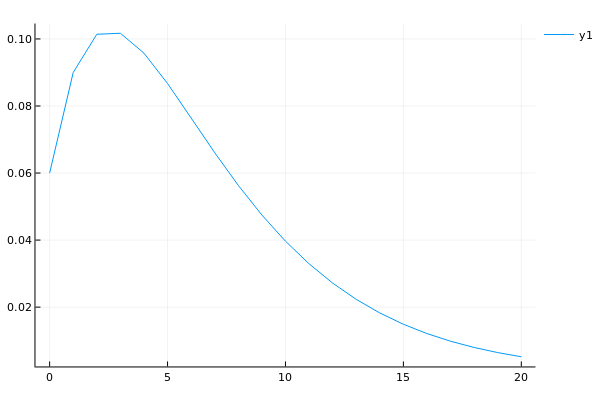
\includegraphics[scale=0.6]{images/1000_problems_in_prob_3_1.png}
\end{figure}


If the two RVs have the same geometric distribution with parameter $p$, $f_X(k) = p(1-p)^ k$, the pmf of their sum becomes

\be\label{2018-12-18:eq1}
f_Z(z) = \sum_{k=0}^z p (1-p)^k (1-p)^{z-k} = p^2 \sum_{k=0}^z (1-p)^z = z p^2 (1-p)^z
\ee


\subsection{Section 3.8, Problem 4}

Now we add $r$ geometric RVs, $X_i$ with the same parameter $p$, and want to show that $Z = X_1 + \cdots + X_r$ has a negative binomial distribution according to

\bee
f_Z(z; r) = {r+z-1 \choose z} (1-p)^z p^r
\eee

Note: Varous books and Wikipedia define the parameters slightly different; the chosen ones are consistent within this entry.

We show this via induction. Start for $r=2$,

\bee
f_Z(z; 2) = {z+1 \choose z} (1-p)^z p^2 = z (1-p)^z p^2
\eee

which equals \eqref{2018-12-18:eq1}. Ok, now for the induction step $r \rightarrow r+1$:

\bee
f_Z(z; r+1) = \sum_{k=0}^z f_Z(k;r) f_X(z-k) = \sum_{k=0}^z {r+k-1 \choose k} (1-p)^k p^r p(1-p)^{z-k}
\eee

Moving all constant terms in front of the sum yields

\bee
f_Z(z; r+1) = p^{r+1}(1-p)^z \sum_{k=0}^z {r+k-1 \choose k} = p^{r+1}(1-p)^z {r+z \choose z}
\eee

where we have guessed (made numerical experiments) in the last equation. The last expression is $f_Z(z; r+1) = {r+z \choose z} (1-p)^z p^{r+1}$ .\qed

Add-on: To show the binomial coefficient magic (Table 174 ``The top ten binomial coefficient identities''  in Concrete Mathematics)

\bee
\sum_{k \leq n} {r+k \choose k} = {r+n+1 \choose n}
\eee

we make use of the addition formula:

\bee
{r \choose k} = {r-1 \choose k} + {r-1 \choose k-1}
\eee

which can be proven by brute-force

\begin{align*}
{r-1 \choose k} + {r-1 \choose k-1} &= \frac{(r-1)!}{k!(r-1-k)!} + \frac{(r-1)!}{(k-1)!(r-k)!} = \frac{(r-1)!(r-k)}{k!(r-k)!} + \frac{(r-1)!k}{(k)!(r-k)!} \\ &= \frac{(r-1)!(r-k+k)}{k!(r-k)!} = \frac{r!}{k!(r-k)!} = {r \choose k} \qed
\end{align*}

Repeated application of the addition formula (to the last term) yields

\begin{align*}
  {5 \choose 3} &= {4 \choose 3} + {4 \choose 2} \\
   \            &= {4 \choose 3} + {3 \choose 2} + {3 \choose 1} \\
                &= {4 \choose 3} + {3 \choose 2} + {2 \choose 1} + {2 \choose 0} \\
                &= {4 \choose 3} + {3 \choose 2} + {2 \choose 1} + {1 \choose 0} + {1 \choose -1}
\end{align*}

which is the desired expansion. \qed


\subsection{Section 3.11, Problem 6}

If $X$ and $Y$ are Poisson-distributed with parameter $\lambda$ and $\mu$, respectively, then their sum $Z = X+Y$ is also Possin-distributed with parameter $\lambda + \mu$. We have $f_X(k) = \lambda^k e^{-\lambda}/k!$ and the pmf of the sum is

\bee
f_Z(z) = \sum_{k=0}^z f_X(k) f_Y(z-k) = \sum_{k=0}^z \frac{\lambda^k e^{-\lambda}}{k!} \frac{\mu^{z-k} e^{-\mu}}{(z-k)!} = \frac{e^{-(\lambda+\mu)}}{z!} \sum_{k=0}^z \lambda^k \mu^{z-k} \frac{z!}{k!(z-k)!}
\eee

The fraction at the end is a Binomial coefficient; $\frac{z!}{k!(z-k)!} = {z \choose k}$ and we obtain

\bee
f_Z(z) = \frac{e^{-(\lambda+\mu)}}{z!} (\lambda + \mu)^z \qed
\eee

The conditional distribution, $f(X|X+Y=z)$ is given as

\begin{align*}
f(X|X+Y=n) &= \frac{f(X=k, X+Y=n)}{f(X+Y)=n} = \frac{f(X=k) f(Y = n-k)}{f(X+Y)=n} = \frac{ \frac{\lambda^k e^{-\lambda} }{k!} \frac{\mu^{n-k} e^{-\mu} }{(n-k)!} }{ \frac{(\lambda + \mu)^n e^{-(\lambda+\mu)}}{n!} } \\ &= \frac{\lambda^k \mu^{n-k} n!}{(\lambda+\mu)^n k! (n-k)!} = {n \choose k} \frac{\lambda^k \mu^{n-k}}{(\lambda+\mu)^n}
\end{align*}

which is a Binomial distribution \qed.

%%% Local Variables:
%%% mode: latex
%%% TeX-master: "journal"
%%% End:
